\documentclass[sigconf]{acmart}

\usepackage{booktabs} % For formal tables
\usepackage{amsmath}
\usepackage{listings}
\usepackage{algorithm}
\usepackage{multirow}
%\usepackage{draftwatermark}
\usepackage[noend]{algpseudocode}
%\SetWatermarkText{Preprint}
\sloppy 

\algnewcommand\And{\textbf{and}}
\lstset{
  language=Python,
  showstringspaces=false,
  formfeed=newpage,
  tabsize=4,
  commentstyle=itshape,
  frame=tb,
  morekeywords={models, lambda, forms}
}
\lstset{
  numbers=left,
  firstnumber=1,
  numberfirstline=true
}

\setcopyright{rightsretained}

\usepackage{comment}
\algrenewcommand\algorithmicprocedure{\textbf{function}}

\begin{document}
\copyrightyear{2019} 
\acmYear{2019} 
\setcopyright{acmlicensed}
\acmConference[EuroSec '19]{12th European Workshop on Systems Security}{March 25--28, 2019}{Dresden, Germany}
\acmBooktitle{12th European Workshop on Systems Security (EuroSec '19), March 25--28, 2019, Dresden, Germany}
\acmPrice{15.00}
\acmDOI{10.1145/3301417.3312497}
\acmISBN{978-1-4503-6274-0/19/03}
\title{Pythia: Identifying Dangerous Data-flows in Django-based Applications}

\author{Linos Giannopoulos}
\affiliation{%
  \institution{Greek Research and Technology Network}
}
\email{lgian@noc.grnet.gr}

\author{Eirini Degkleri}
\affiliation{%
  \institution{Greek Research and Technology Network}
}
\email{degleri@noc.grnet.gr}

\author{Panayiotis Tsanakas}
\affiliation{
  \institution{National Technical
  University of Athens}
}
\email{panag@cs.ntua.gr}

\author{Dimitris Mitropoulos}
\affiliation{%
  \institution{Greek Research and Technology Network}
}
\email{dimitro@grnet.gr}

\renewcommand{\shortauthors}{L. Giannopoulos et al.}

\begin{abstract}
Web frameworks that allow developers
to create applications based on design
patterns such as the
{\it Model View Controller} ({\sc mvc}),
provide by default a number of security checks.
Nevertheless,
by using specific constructs,
developers may disable these checks
thus re-introducing classic application
vulnerabilities such as Cross-site Scripting
({\sc xss}) and Cross-Site Request Forgery
({\sc csrf}).
Framework-specific elements including
(1) the complex nature of these applications,
(2) the different features that they involve
(e.g. templates),
and (3) the inheritance mechanisms
that governs them,
make the identification
of such issues very difficult.

To tackle this problem,
we have developed {\it Pythia},
a scheme that analyzes applications
based on the {\it Django} framework.
To identify potentially dangerous
data flows that can lead to
{\sc xss} and {\sc csrf} defects,
Pythia takes into account all the
aforementioned elements and employs
ideas coming from standard
data-flow analysis and taint tracking schemes.
To the best of our knowledge,
Pythia is the first mechanism
to consider framework-specific
elements in its analysis.
We have evaluated our scheme
with positive results.
Specifically,
we used Pythia to examine five open-source
applications that are currently in production
and have thousands of users
including an e-voting service,
and a web-based translation
management system.
In four cases we have identified dangerous paths
that in turn led to vulnerabilities.
Notably,
in many cases the paths involved the
particular features of Django-based
applications e.g. templates.
\end{abstract}

\begin{CCSXML}
<ccs2012>
<concept>
<concept_id>10002978.10003022.10003026</concept_id>
<concept_desc>Security and privacy~Web application security</concept_desc>
<concept_significance>500</concept_significance>
</concept>
<concept>
<concept_id>10011007.10011074.10011099.10011102</concept_id>
<concept_desc>Software and its engineering~Software defect analysis</concept_desc>
<concept_significance>500</concept_significance>
</concept>
</ccs2012>
\end{CCSXML}

\ccsdesc[500]{Security and privacy~Web application security}
\ccsdesc[500]{Software and its engineering~Software defect analysis}

\keywords{Data-flow Analysis,
Application Security, Templates,
Unsanitized Output,
Cross-site Scripting,
Cross-Site Request Forgery, Django}

\maketitle

\section{Introduction}
Development frameworks based on existing
programming languages and architectural patterns,
have become one of the most
widespread vehicles to create web
applications.
Such frameworks include by default
security features to assist
developers write secure code without
introducing vulnerabilities such as
{\sc sql} injection,
Cross-Site Scripting ({\sc xss}) and
Cross-Site Request Forgery ({\sc csrf}).
In this way,
developers do not have to re-invent the wheel every time they needed to examine
user input or sanitize the output of their
application.

However,
on many occasions developers need
to disable such features to
allow for specific functionalities.
This can re-introduce the
aforementioned vulnerabilities.
In addition,
the complex nature of the
frameworks~\cite{OPM15}
and the various features that they offer
can make the identification of
such defects a difficult task.

{\it Django} is a popular Python-based web
framework that follows the Model
Template View ({\sc mtv}) design pattern,
an adaptation of the
Model View Controller ({\sc mvc})
architectural pattern~\cite{GLH03, BD04}.
In a Django-based application
% the {\sc mtv}
% \textcolor{blue}{this is framework-specific
% and it is not mentioned in the
% architectural pattern} context
there is an object-relational mapper
({\sc orm}) that mediates between data models
and a relational database ({\it model}).
There is also a system for
processing {\sc http} requests with
a web templating system ({\it view}),
and a regular-expression-based
{\sc url} dispatcher.
Finally,
both patterns provide several features that
can be used to enhance an application such
as {\it templates} and {\it decorators}.
% \textcolor{blue}{Also Django-specific,
% the arc pattern doesnt describe these}.

A potential risk emerges when developers
disable the security checks that the
framework provides,
especially within these features.
In addition,
such issues are difficult to identify because
of inheritance mechanisms supported
by the frameworks,
e.g. a template inherits another one with
disabled security checks.
Notably,
existing mechanisms are not designed
to detect such dangers.

\begin{figure*}[t]
    \begin{center}
        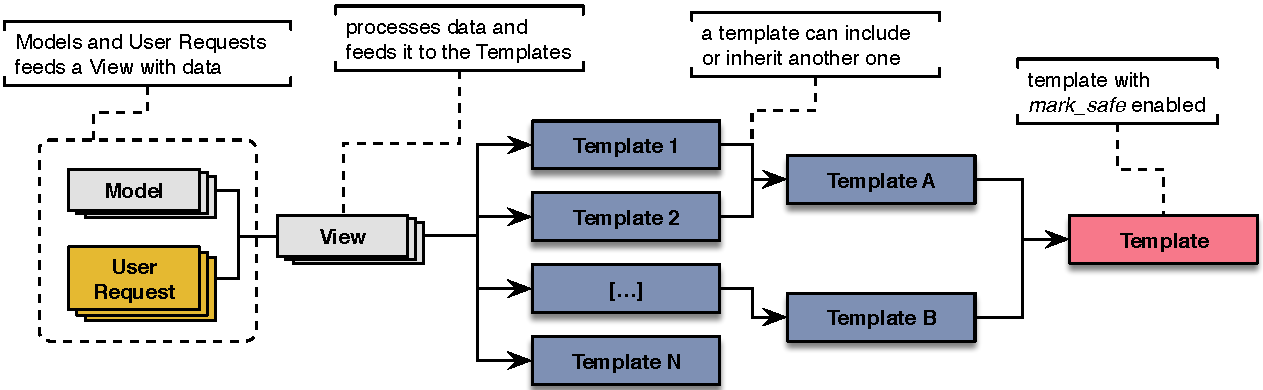
\includegraphics[scale=0.75]{defect_2.pdf}
        % \vspace{-2mm}
        \caption{A potentially vulnerable Django
        {\tt template} is included by various templates which in turn are utilized by Django
        {\tt Views}}\label{fig:defect}
    \end{center}
    % \vspace{-3mm}
\end{figure*}

To address this issue,
we have developed
{\it Pythia},\footnote{In
ancient Greece, {\it Pythia}
was the name of the high priestess
of the Temple of Apollo at Delphi
who also served as the oracle.}
a mechanism that analyzes
Django-based applications to identify
potentially dangerous data paths.
In particular,
it checks if dangerous code constructs
(i.e. the ones used to bypass the security checks provided by the framework)
are included in an application.
Then,
by performing data-flow analysis
it examines all critical application
parts to identify if any data that
may incorporate user input reaches
the constructs identified in the
first step.
Note that,
Pythia searches for potentially
dangerous data flows.
That is,
an alert does not necessarily involve
an existing hazard.
However,
such alerts can be helpful to
the developer in the future as we
further explain in our ``Evaluation"
section (\ref{sec:eval}).

Our mechanism borrows some of
the standard ideas
(Abstract Syntax Tree ({\sc ast}) analysis)
and terms
({\it sources} and {\it sinks})
of other data-flow
analysis~\cite{LL05, JKK06, DH14}
and taint tracking
schemes~\cite{VFJKKV07, PMP11, SLMS14}
employed to identify
web application defects.
Nevertheless,
it goes one step further and takes
into account the complicated architecture
and the various mechanisms
(inheritance) and features (templates)
of Django-based applications.
To explore paths in such applications
Pythia follows a novel way of
analysis that can be applied
in other similar contexts such
as {\it Laravel}~\cite{laravel},
an {\sc mvc}-based framework used to
create applications in {\sc php}.

We have evaluated Pythia by
examining four,
large,
open-source applications
with thousands of users including
an e-voting service~\cite{zeus-jets},
a cloud service,
and a web-based translation
management system~\cite{weblate}.
In all cases we have identified
corresponding vulnerabilities and
notified the developers.
Apart from the straightforward
{\sc xss} vulnerabilities
(where user input may reach a
sink in a view),
Pythia identified many paths
that involved the particular features of
Django-based applications such as templates.

Three of the applications were patched
hence we provide further details about them.
Following responsible disclosure practices,
we do not reveal the name of
the fourth application and we will
do so once the issue is fixed.

% By using such frameworks
% developers can easily design
% applications and 
% attempt to eliminate writing boilerplate
% code that was a tedious and 
% repetitive task for developers. 

% At the same time,
% the security community had to
% combat several popular 
% vulnerabilities such as {\sc sql} injection,
% Cross-Site Scripting ({\sc xss}) and
% Cross-Site Request Forgery ({\sc csrf}). 
% As a result,
% the framework maintainers started to incorporate the necessary 
% security features within the frameworks
% so that developers were able to 
% access them directly instead of
% reinventing the wheel every time
% they wanted to sanitize user input.

%Some of these components were built with security in mind. 
% Object-Relational Mapping ({\sc orm}), is also a technique that was 
% created with security in mind. It aims to abstract the communication with 
% relational databases and so as a side effect, the database queries are 
% generated by the {\sc orm} itself. 
% As a result, there is little room for error from the developer's side.
% Of course, that puts the burden of security upon the {\sc orm} developers 
% but it also gives the community the advantage of having to maintain 
% and audit only a handful of {\sc orm}s.

% Citing a paper~\cite{OPM15}.
% % MVC elements here, maybe?
\section{Background}
\label{sec:background}

The Model View Controller 
({\sc mvc}) architectural
pattern~\cite{GLH03, BD04}
is one of the most widespread design
patterns used for developing user interfaces. Specifically,
it divides an application into three
basic parts that are interconnected.
The {\it model} is the application's
data structure which is independent
of the user interface and it directly
manages the data of the application.
A {\it view} can be any output
representation of information and finally,
the {\it controller}
accepts input and converts it into
commands for the model or view.
Currently,
there are thousands of web applications
that are implemented based on the {\sc mvc}
pattern.

Our research focuses on applications
that follow an adaptation of the
{\sc mvc},
namely the Model Template
View ({\sc mtv}) pattern.
In the {\sc mtv} context
there is an object-relational mapper
({\sc orm}) that mediates between data models
and a relational database (model).
There is also a system for
processing {\sc http} requests with
a web templating system (view),
and a regular-expression-based
{\sc url} dispatcher.
Templates are parts of the
client-side code and are employed by views.

Django is a Python-based Web framework
that follows the {\sc mtv} pattern
and allows developers to build
large applications in an easy way.

Even though {\sc mvc} facilitates
structured code,
it introduces a complexity that
may lead to inconsistencies~\cite{OPM15}.
In addition,
its multiple features and tangly
structure makes it hard to manually
identify vulnerabilities such as
{\sc xss} or {\sc csrf}.
 
In particular it is difficult to trace tainted data within the 
application, because in addition to the standard components of 
the architecture, other elements (i.e. templates), which follow 
inheritance relations, are in place. 
At the same time, an automated tool can relatively easy track 
data  flows due to the formalization of coding structure that 
web frameworks have brought. 

\paragraph{MVC in Django}
Django ~\cite{django} is a Python based web framework, that is 
widely used by the community since it offers many features
for easy and quick development and because of the  
increasing growth of Python ~\cite{python_trend}.
It follows a Model Template View ({\sc mtv}) or ({\sc mvt}) 
architectural pattern ~\cite{Holovaty:2009:DGD:1572516}, 
\cite{django_mvt}, which is slightly different than the 
standard {\sc mvc}. 

Django's {\tt Template}, is a part of the client-side 
and relates to the {\tt View} in {\sc mvc} as it controls what is 
displayed to the user. The {\tt Model}, has the same role in the 
{\sc mvc} and {\sc mvc} and is part of the server-side.  
Correspondingly Django framework incorporates the {\tt View} and the 
application logic, which relates to the standard {\tt Controller}, 
since it is responsible for the communication between the 
{\tt Template} and the {\tt Model}. 





\section{Vulnerability Inheritance in Django-based Applications}
\label{sec:motivation}
\vspace{-0.5mm}

Development frameworks enforce security mechanisms such as the 
sanitization of {\sc html} output by default.
In this way, certain characters
(e.g. '{\tt <}' and '{\tt \&}')
are not interpreted as special
control characters.
However,
the frameworks also
allow programmers to
bypass such mechanisms to support
specific use cases which 
in turn, can lead to serious
vulnerabilities including {\sc xss} and {\sc csrf}.

A serious issue emerges when this bypassing
happens in {\it templates}, 
a feature that provides a way to generate {\sc html} dynamically.
Templates are supported by several frameworks
including Django and Laravel.
In general,
templates contain static parts of the 
desired {\sc html} output,
together with some special 
syntax describing how the dynamic
content will be inserted.

When developers insert
{\sc html} content into a template,
they need to mark it as ``safe", 
so that the framework itself
treats it as such, 
and avoid escaping {\sc html} characters.
In this case developers have to be sure about the
origins of the content
because if the content 
includes user input,
attackers can perform an 
{\sc xss} attack.

To track such a vulnerability is not trivial
because templates can either
{\it include} or {\it inherit}
other {\tt templates}.
Hence,
it is difficult to find which
views are affected
by a potentially vulnerable template.
Figure~\ref{fig:defect},
highlights this issue,
i.e. a template that marks content
as safe is included by multiple other
ones within the application.
In turn, 
these templates are used by different 
views that process content either from user 
input, or loaded from the model. 

Another issue occurs when
developers use the 
{\tt @csrf\_exempt} decorator to disable 
{\sc csrf} protection in Django
views ~\cite{csrf_exempt}.
Specifically,
Django allows developers to
inject a {\sc csrf} token 
for every form rendered and then
expect the client 
to supply this token with the
corresponding {\sc post}  request.
This mechanism is disabled when the {\tt @csrf\_exempt} 
feature is used.

To identify the aforementioned issues
during a code review,
security experts have to find all
the occurrences 
of the different features and
track which views are affected manually.
Such a task could even be performed
using {\tt grep} command.
However this would require an
exhaustive  and repetitive search
from the security expert's side.

Additionally, 
tracking the various intermediate entities that inherit 
such properties is not an easy task in modern,
large applications. 
Thus,
some level of automation is
needed to cope with 
large code-bases.
Our approach provides a way to
automatically discover 
data flows when such features
are employed and 
warn security engineers
about potentially vulnerable paths.

\vspace{-2mm}

\section{Approach}
\label{sec:approach}

This work describes {\it Pythia},
an approach that analyzes applications,
to identify data-paths
which involve dangerous constructs such
as the ones described in Section~\ref{sec:motivation}.
To do so,
Pythia analyzes an application's
views and templates,
leaving out models as they do not hold any relevant information.
Figure~\ref{fig:arch} presents the basic steps performed by our approach:
First,
Pythia searches for specific constructs,
which we call {\it sinks},
marking any affected templates and then,
examines views to identify
\textbf{(1)} if untrusted data can reach
the elements identified in the first step,
\textbf{(2)} if other sinks are being used by the views.

\vspace{-2mm}

\begin{figure}[t]
    \begin{center}
        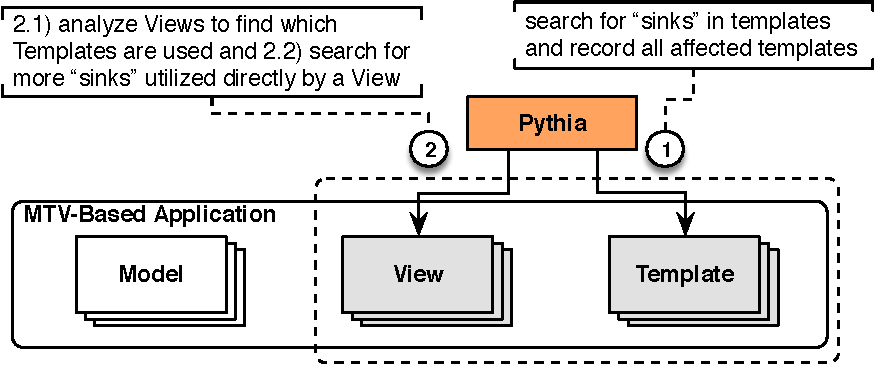
\includegraphics[scale=0.45]{MVC_and_Pythia_2.pdf}
        \vspace{-3mm}
        \caption{In the Model Template View ({\sc mtv}) Context, {\it Pythia} focuses on {\tt Views} and {\tt Templates}.}\label{fig:arch}
    \end{center}
    \vspace{-6mm}
\end{figure}

\subsection{Sinks}
\label{sec:sinks}

A sink method depicts a coding construct
where the hazard might take place~\cite{MLPK17}.
In our case,
a sink involves an invocation that bypasses
the default security mechanisms of a Django
Application.
In such an application we can divide sinks
into two categories,
namely:
{\it in-view sinks},
and {\it template sinks}.
The first category
only affects a particular {\tt View},
while the second on involves templates
that may affect all the views that use them. 

{\it Template Sinks} involve Django filters
such as {\tt safe} and {\tt safeseq},
and tags such as {\tt autoescape}.
The {\tt autoescape} tag,
controls the auto-escaping effect of a code block.
When disabled (set to {\tt off}),
it is equivalent to marking all variables
inside that code block as ``safe".
Escaping concerns dangerous characters
such as '{\tt <}', which in turn is 
converted to '{\tt \&lt;}' and more.
Furthermore,
filters including {\tt safeseq} and
{\tt safe} dictate that a variable
does not require further {\sc html} escaping
before it becomes part of  the output.

{\it In-view Sinks} include {\it decorators}
such as {\tt @csrf\_exempt} and functions
invocations that can lead to {\sc xss}
defects when used in an improper manner
(e.g. {\tt mark\_safe}).

To trace dangerous data flows,
Pythia expects as input two lists which in turn
include the constructs of each category.
The lists, can easily be expanded with more methods 
depending on the needs of the developer,
thus providing flexibility to track other 
application / project-specific filters
or decorators.

When Pythia identifies a sink,
it then examines the application
for potential sources,
i.e. variables that hold data that
can reach the sink.
Notably,
such data can come from a {\tt Model}
or a user request
(e.g. {\tt request.GET.get()}).
In the upcoming section we discuss
how Pythia examines the various data paths
of an application.

\begin{algorithm}[b]
\caption{Searching for Dangerous Flows}
\label{alg:explore}
\begin{algorithmic}[1]
\State {\bf INPUT} $TS$: template sinks
\State {\bf INPUT} $IS$: in-view sinks
\State {\bf INPUT} $url\_conf$: the {\tt urlpatterns} object containg all URLs
\Function{analyze}{$TS$, $IS$, $url\_conf$}
\State $S \gets set();$

\State $T \gets getTemplates();$
\Comment{ Stage 1 }
\State $paths[];$

\ForAll{$t \in T$}
    \State $t.walk(TS, paths[], t.root, t.name);$
\EndFor
\State $V \gets getAllViews(url\_conf);$
\Comment{ Stage 2 }
\ForAll{$v \in V$} 
    \If{$v.invokes(IS)$}
        \State $S.add(v);$
    \EndIf
    \ForAll{$p \in paths[]$}
        \If{$v.renders(p)$}
            \State $S.add(v, p);$
        \EndIf
    \EndFor 
\EndFor
\EndFunction
\end{algorithmic}
\end{algorithm}

\subsection{Application Analysis}
\label{sec:analysis}

Algorithms~\ref{alg:explore}
and~\ref{alg:paths} illustrate
how Pythia examines a Django application.
First,
our approach retrieves all project templates
and generates their corresponding
Abstract Syntax Trees ({\sc ast}s).
Then,
starting from the root node of each {\sc ast},
it recursively traverses all children
nodes searching for variables that
reach a sink method.
This process starts in line 9
of Alg.~\ref{alg:explore} and continues
in Alg.~\ref{alg:paths}.
Specifically,
when Pythia identifies a sink,
it marks the template as potentially
dangerous (Alg.~\ref{alg:paths}, line 9).
If the current template extends or
includes another one,
the approach goes on to examine
the other template too
(Alg.~\ref{alg:paths}, lines 10-13).
In this way it creates a path that
is recorded when a sink is found.
When a dangerous path is found, the current node 
and the template ancestry are kept in a key-value store in 
order to be cross-examined in the second stage.

When the first part finishes,
Pythia analyzes the views of the application
and extracts all decorators.
Then,
it traverses the {\sc ast} of each {\tt View}
to identify the templates that are being used
and the data that each template requires 
to render the page.
Finally,
the results are 
being cross-examined in order to find
unsafe data paths.

\vspace{-2mm}

\begin{algorithm}[b]
\caption{Exploring Paths}
\label{alg:paths}
\begin{algorithmic}[1]
\State {\bf INPUT} $TS$: template sinks
\State {\bf INPUT} $paths[]$: a list holding all
potentially tainted paths
\State {\bf INPUT} $node$: current {\sc ast} node
\State {\bf INPUT} $origin$: template ancestry
\Function{walk}{$TS$, $paths[]$, $node$, $origin$}
\ForAll{$subnode \in node.nodelist$}
  \If{$subnode.isVariable()$}
    \If{$subnode.invokes(TS)$}
      \State $paths[] \gets subnode, origin;$
    \EndIf
  \ElsIf{$subnode.isExtendsNode()$}
    \State{$walk(TS, paths, subnode, subnode.extended\_tmplt)$}
  \ElsIf{$subnode.isIncludeNode()$}
    \State{$walk(TS, paths, subnode, subnode.included\_tmplt)$}
\EndIf
\EndFor
\EndFunction
\end{algorithmic}
\end{algorithm}

\subsection{Resolution of Paths}
\label{sec:output}

The output of Pythia is based on the
category of the sink identified.
In the case of a decorator
(i.e an in-view sink such as
{\tt \@csrf\_exempt}),
the output contains:
(1) the {\sc url} under
which the potentially vulnerable
view resides,
(2) the module where the view is defined
(the last component of the module is the view's name), 
and (3) which decorators were used on it.

If a dangerous function is identified within a view,
Pythia returns (1) the view's corresponding
{\sc url} (e.g. /users/<id>/),
(2) the module where the view is defined
alongside with the line under where
the function was invoked,
(3) the function's name,
and (4) the variable it was ran upon.

For template sinks,
Pythia's output includes all views that render,
directly or indirectly,
a template that uses the list of
unsafe filters and tags.
Also,
it contains the module and the line where
the view is defined,
the ancestry path to reach the dangerous template,
the filter that was applied,
the variable itself,
and the variable's context.
\footnote{The term context is used to describe all variable aliasing / assignments
within the current scope, until a dangerous filter invocation is reached.}
Note that the context information is needed
to track the data provided from the view to
the template until they reach the sink.

Furthermore,
in case a specific template containing sinks
does not resolve to a view,
the path to the sinks is still part of the output.
In this manner,
a security expert can manually resolve
the given template until the source
of the data is found.
An example where the full path is not
resolved is when a template is used
for the rendering of a form inside a template.
Currently,
Pythia does not go through form definitions
to find template invocations.

\vspace{-1.5mm}

\subsection{Output Filtering}
\label{sec:filtering}

Pythia outputs a number of potentially
dangerous data paths.
This means that a part of a path
may appear in other several paths.
In addition,
a template that marks output
as safe may be included by multiple
templates.
In such occasions the output of
the tool may include recurring information
with duplicated elements.

To reduce the volume of such instances
we apply filters that make the output
more comprehensive and easy to use.
For instance,
we enumerate the views that end up
using a template including {\tt safe} tags
and let the user explore their names as a
second step.

\vspace{-1.5mm}

\subsection{Implementation Details}
\label{sec:implementation}

As we described earlier,
Pythia requires the {\sc ast} of a template.
To generate this {\sc ast},
Django requires a running environment.
This is because Django needs to resolve
user-defined components (e.g. custom filters)
and its own defaults (e.g. for loops, variable aliasing).
Other operations such as the analysis of a view's
module are realized statically using Python's
{\sc ast} package.

This design decision, to divide the implementation
between purely static and processes that require
Django's run-time to be setup has certain
assets and liabilities.
Using a purely static approach,
one can easily use the tool on many projects
without having to configure their dependencies
and even run it during a project's continuous
integration as another security test.
However,
with the hybrid approach one can gain the
advantage of having the ability to use
certain aspects of Python's and Django's
run-time and exploring paths that
otherwise would not be possible to explore. 

Regarding further implementation details, 
Pythia supports both Python 2.x and 3.x
versions and Django 1.8.x until 1.11.x. Versions 
before 1.7.x, are not supported as they have a
vastly different internal representation
of the {\sc ast} node classes.
\vspace{-1.5mm}

\section{Evaluation}
\label{sec:eval}

We have applied Pythia on five
different open-source,
Django projects.
Note that many Django projects
involve Jinja~\cite{jinja} templates
and Pythia does not currently
analyze such templates.
Hence,
we focused on projects that only
employ Django templates.

In four projects we found vulnerabilities.
We have reported the defects to
the developers of each project and in
all cases patches were introduced.
Notably,
all applications have thousands of users.

Table~\ref{tabular:apps} presents the results
of our evaluation.
Specifically,
we show the number of each vulnerability
that Pythia identified for each application,
and provide a high-level
description of the impacts.
In the following,
we provide further details
regarding the applications and the defects we found.
Pythia did not report any defects for
Misago~\cite{misago},
a forum application written in Python.

\begin{center}
\begin{table}[b]
  \caption{Evaluation Results}
  \vspace{-3mm}
  \begin{tabular}{p{1.8cm}| l | lp{1.6cm}|lp{1.6cm}}
    \hline
     \multirow{2}{*}{\textbf{Application}} &
        \multirow{2}{*}{\textbf{Version}} &
        \multicolumn{2}{c|}{\textbf{XSS}} &
        \multicolumn{2}{c}{\textbf{CSRF}} \\ 
        & & {\#} &  {\it Impacts} & {\#}  & {\it Impacts} \\ \hline
        $\sim$okeanos & - & 3 & Privilege Escalation & 0 & - \\
        \hline
        Zeus & - & 1 & Privilege Escalation & 2 & Password Reset \& {\sc d}o{\sc s}  \\ \hline
        ViMa & 2.2 & 0 & - & 9 & {\sc vm} Manipulation \\ \hline
        Weblate & 3.3 & 1 & Privilege Escalation & 0 & - \\
    \hline
  \end{tabular}
  \label{tabular:apps}
\end{table}

\end{center}

\vspace{-6mm}

\subsection{$\sim$okeanos}
\label{sec:okeanos}

$\sim${\it okeanos}~\cite{okeanos} is an
an IaaS (Infrastracture as a Service)
that has been in production since early 2012.
It offers cloud computing services to
the Greek and the European research and academic community,
and involves thousands of users.

In the case of $\sim$okeanos,
Pythia identified an {\sc xss} vulnerability
very similar to the one described in
	Section~\ref{sec:motivation}.
Specifically,
one of the application's views
includes a template named
{\tt project\_application\_form.html}:

\vspace{0.8mm}
\begin{lstlisting}[language=Python, basicstyle=\footnotesize\ttfamily]
 template_name = '/projects/project_application_form.html'
\end{lstlisting}
\vspace{0.8mm}

\noindent
At some point,
the {\tt View} utilizes the template to render a form
that incorporates data stored in the database.
However,
the data are initially provided by users
through another form.
In turn,
the template above
includes another one named
{\tt form\_field.html}:

\vspace{0.8mm}
\begin{lstlisting}[language=html,basicstyle=\footnotesize\ttfamily]

    
        
    

\end{lstlisting}
\vspace{0.8mm}

\noindent
The sink occurs in {\tt form\_field.html}
where every field of a form is marked as safe
for output (line 14):

\vspace{0.8mm}
\begin{lstlisting}[language=html,basicstyle=\footnotesize\ttfamily]

<div class="form-row"
    with-errors
    with-hidden">
      {{field.errors}}
      <p class="clearfix
         required">
         {{field.label_tag}}
         {{field|safe}}
         <span class="extra-img">&nbsp;</span>
            
                <span class="info">
                    <em>more info</em>
                    <span>{{field.help_text|safe }}</span>
                </span>
            
         </p>
    </div>

\end{lstlisting}
\vspace{0.8mm}

\noindent
The above can lead to an {\sc xss} vulnerability~\cite{MLPK17},
i.e. attackers can inject malicious scripts
that are first stored on the database
of the application
and then run in the browser of other users
(including administrators),
thus stealing their cookies.

\vspace{-1.5mm}

\subsection{Zeus}
\label{sec:zeus}

{\it Zeus}~\cite{zeus-jets, zeus}
is an e-voting application
that has been in production
since late 2012 and
has been used in more than 500
real-world elections involving
more than 55,000 voters~\cite{pnrmx-del}.

The {\sc xss} vulnerability
that was discovered in Zeus is very
similar to the one described earlier.
An interesting observation
was that the view that included
the template with the sink,
was not accessible through the
application's
{\sc gui} (Graphical User Interface).
However,
after examining the code of the application,
attackers could reach the view through
a specific {\sc url}.
Hence,
a vulnerability scanner that examines
a running instance of the application
would not discover the vulnerability.
Contrary to such scanners,
Pythia's
ability to map {\sc url}s to views
(as described in
Subsection~\ref{sec:implementation})
led to the identification of the
dangerous path.

Apart from the {\sc xss} defect,
Pythia identified two
to {\sc csrf} vulnerabilities:
one that can be employed to reset
passwords and another that
can be a denial of service attack vector.

Specifically,
in the application version that we examined,
the password reset functionality was
accessed through a {\sc get} request from
a specific {\sc url} which incorporated
the {\sc id} (i.e. a number) of a user
as a parameter.
A valid attack scenario in this case,
would be to host a website that sends
{\sc ajax} requests to the application
to reset every password.
Given that the users' {\sc id}s
are stored in a sequential way
in the database this is easy to accomplish.
This would cause organizational mess
during an election since the administrator
or anyone else would not be able to log-in.

Missing {\sc csrf} protection on
another {\sc post} form could lead to
a Denial of Service ({\sc d}o{\sc s})
attack through a {\sc csrf} attack.
In particular,
attackers could host a website,
lure victims to it,
and submit the form multiple times
through the victim's browser.
The above would lead to resource drain
due to the required computing resources
needed by the attacked endpoint.

\vspace{-1mm}

\subsection{ViMa}
\label{sec:vima}

{\it ViMa} (Virtual Machines)~\cite{vima},
provides to the Greek academic community
access to shared computing and network resources that can be used
for production purposes.
Currently,
it is used by a hundreds of researchers
and practitioners.

Pythia identified numerous
{\tt @csrf\_exempt} decorators
that can lead to 9 types of
{\sc csrf} attacks.
Through these attacks an attacker
can perform different actions including:
rebooting a virtual machine of another user,
shutting it down and destroying it. This attack
requires that the victim is lured to browse to a malicious
website that performs these actions using the
victim's credentials, leveraging the lack of
{\sc csrf} protection.
For instance,
the following decorator
allows an attacker to reboot
a virtual machine of another user:

\vspace{0.8mm}
\begin{lstlisting}[language=Python, basicstyle=\footnotesize\ttfamily]
@login_required
@csrf_exempt
@check_instance_auth
@check_admin_lock
def reboot(request, cluster_slug, instance):
    cluster = get_obj_or_404(Cluster, slug=cluster_slug)
    [...]
\end{lstlisting}
\vspace{-2mm}

\subsection{Weblate}
\label{sec:weblate}
\begin{comment}
https://github.com/WeblateOrg/weblate/blob/d84dfdbdfaba0d31588fd3bc9253e6d75d03e644/weblate/trans/views/basic.py#L91-L129
\end{comment}
{\it Weblate}~\cite{weblate} is a web-based
translation management system.
It is  used for translating many free
software project as well as commercial ones,
including
{\it phpMyAdmin}~\cite{phpma} and
{\it Debian Handbook}~\cite{dhbk}.

In the case of Weblate,
user data stored in the database
were being marked as safe
even before being sent to the view's corresponding template (in-view sink).
In particular,
the name of a project is provided by a user.
Then,
this information is marked as safe by
the application and is included on
the output. {\footnote{\url{https://github.com/WeblateOrg/weblate/blob/d84dfdbdfaba0d31588fd3bc9253e6d75d03e644/weblate/trans/views/basic.py\#L91-L129}}}
This issue led to stored {\sc xss} attacks
that could be used to elevate any user's privileges to the ones of an administrator.

\subsection{False Positives and Negatives}
\label{sc:fa}

A potentially dangerous path
may involve a source that will
not include user data
e.g. a variable that is instantiated
by retrieving data from the database
and in turn the data are auto-generated
by the application.
Pythia will report the path above
producing a false alarm.
An alarm like this was produced
when we examined $\sim$okeanos.
Specifically,
the path involved the terms and
conditions of $\sim$okeanos.
which are marked as safe by
the template when they are
displayed to the user.
However,
such information is not useless.
After seeing such a path,
a developer can note it down and
be careful in the future regarding the
identified sink.

In general,
false positives in related mechanisms
(either data-flow analysis or
taint tracking techniques)
is a known issue~\cite{ME07, MLPK17}.
Pythia though should be seen
as an assistant for developers
who want to have a thorough
security perspective
of their application,
and not as a vulnerability detector.

A false negative may appear in the following
way: consider a {\tt mark\_safe} construct
that exists in a function invoked by a view,
Pythia will not report this case because
it does not examine the code of the invoked functions.
However, we can perform a more in-depth analysis and
include such cases too.

\section{Related Work}
\label{sec:rel}

Pythia is related to
various approaches that
have been developed to identify web 
application vulnerabilities
either through {\it static data-flow
analysis} or {\it dynamic taint tracking}.
We describe how each one operates,
and outline its main characteristics

Livshits et al.~\cite{LL05}
statically analyzes the {\sc cfg}
(Control Flow Graph) of a Java application
to identify variables
that carry user input and check if
they reach a sink method.
In this way they detect
possible {\sc sql} injection and
{\sc xss} defects.
{\it Pixy}~\cite{JKK06} is an open source tool that examines {\sc php} scripts
in a similar manner.
In Pixy,
rules can appear in the source of the
program in the form of annotations.
Dahse and Holz~\cite{DH14} have introduced a
refined type of data-flow analysis to
identify second-order vulnerabilities.
Note that vulnerabilities of this kind
occur when an attack payload
is first stored by the web application
on the server-side and then later on used
in a security-critical operation.

Vogt et al.~\cite{VFJKKV07} have
developed a taint tracking scheme
which operate on the server-side at runtime.
Their mechanism tracks sensitive
information at the client-side
to ensure that a script can send
sensitive user data only to the
site from which it came from.
In this way they prevent {\sc xss}
attacks that may attempt to send
the user's cookie to a malicious site.
Stock et al.~\cite{SLMS14} use
taint tracking to prevent
{\sc dom}-based {\sc xss} attacks.
Specifically, it employs a taint-enhanced JavaScript engine that
tracks the flow of malicious data.
To prevent an attack,
the scheme uses {\sc html} and JavaScript
parsers that can identify the generation of code which in turn comes from tainted data.
{\sc wasc}~\cite{NLC07} and
{\sc php} {\it Aspis}~\cite{PMP11}
apply further checks when it is
established that tainted data have
reached a sink.
In particular,
{\sc wasc} analyzes {\sc html}
responses to examine
if there is any data that contains malicious
scripts to prevent {\sc xss} attacks.
{\sc php} Aspis,
associates tainted data with metadata
such as the propagation path to
prevent {\sc sql} injection and
{\sc xss} attacks in {\sc php} applications.

% To increase automation, static analyzers are used to detect coding and/or syntax errors, examine code structure and thwart security vulnerabilities. {\sc OWASP} project has published WAP - Web Application Protection Project ~\cite{owasp_wap}, which aims to detect and even correct input validation vulnerabilities for web applications written in {\sc php}, predicting false positive results. 

There is a number of static analysis
mechanisms that are used to analyze Python
programs and applications that are
also related to Pythia.
Libraries such as
{\it Pylint}~\cite{pylint},
{\it Flake8}~\cite{py_flake},
and {\it Django Lint} ~\cite{django_lint}
are popular quality checkers that report
common programming errors such as code
smells and provide simple refactoring
suggestions.
Security wise,
the most widely used
python static analyzer is
{\it Bandit} ~\cite{bandit},
which is being actively maintained.
However,
it does not provide great insights
when analyzing large Django projects.
This is because it analyzes {\sc ast}s 
searching for dangerous code
constructs without any further analysis.
As a result,
it generates numerous false alarms.
{\it Python Taint}
({\sc pyt})~\cite{pyt} extends the
functionality of Bandit and performs
data-flow analysis thus providing more
precise results.
Nevertheless,
{\sc pyt} does not take into account
elements such as templates and
mechanisms such as inheritance.
Hence,
it cannot address vulnerabilities
like the ones described in
Section~\ref{sec:motivation}.
In addition,
it does not resolve {\sc url}s
to views to provide a detailed path.
Contrary to the above techniques,
Pythia takes into account all the
novel features of a modern,
Django-based application including
templates and decorators.
In this way it identifies vulnerabilities
that other tools fail to do so.

% Similarly Python Taint (PYT) ~\cite{pyt} is a promising static analysis tool, based on Control Flow Graph (CFG), and dataflow analysis. Although it provides adaptors for Python frameworks, it can only support analysis for Django on a superficial level, since it cannot resolve URLs to views and analyze templates, for which the runtime environment is necessary. On the contrary, as described in \ref{sec:implementation}, Pythia fosters this by design. 

% Check and improve this! 
% To summarize, this work focuses on an analyzer tailored for Django's environment, which aims to provide developers and security experts with information regarding potential sinks, leveraging on Python abstract syntax tree.  
% The inducement towards the Django framework is that although it considered to supply developers with many security mechanisms \cite{django_sec}, there are cases where either developers do not make use of these mechanisms ~\cite{nguyensecurity}, or the framework itself has vulnerabilities ~\cite{django_cve}. 
% Additionally, based on our research there is not a similar solution to {\it Pythia}, meaning that there is not an open-source tool targeted to Django based applications that exposes dangerous filters, in-view marked safe variables and decorator invocations.


\section{Conclusions}
\label{sec:conc}

Modern web frameworks intent to
assist developers by enabling
security features by default.
Nevertheless,
the negligent bypassing of these
measures can compromise 
the security of an application.
Furthermore,
the complex architecture of
{\sc mvc}-based applications
makes it hard to identify such hazards.
Pythia,
aims to assist developers and
security experts to identify
such issues within large code bases
and in an easy manner.
Furthermore,
our evaluation results indicate
that Pythia can be used to examine
applications in production and with
thousands of users.

Pythia is the first mechanism
that takes into account features
such as templates and their inheritance.
Notably,
the approach behind Pythia can be
applied to different contexts
such as the Laravel framework which
runs on {\sc mvc}-based applications
written in {\sc php}
(see also Section~\ref{sec:motivation}).

Future work on our mechanism
involves the creation of visualizations
based on the tool's output and the
application of further checks
when a dangerous path is identified
in a similar to
{\sc wasc}~\cite{NLC07} and
{\sc php} Aspis~\cite{PMP11}
(see Section~\ref{sec:rel}).

% \subsection*{Code Availability}
% Pythia's source code is open source and
% can be reached through the
% following {\sc url}:

% \subsection*{Acknowledgements}
% This work was supported by the
% {\sc certcoop} project,
% funded by the European Union's
% Connecting Europe Facility Telecom Call
% 2016 with Proposal Code
% 2016-{\sc el}-{\sc ia}-0123
% (Cyber Security).

\noindent
{\bf Acknowledgements.}
This work was supported by the European Union's Connecting
Europe Facility ({\sc cef}) Work Program 2016 under grant agreement
{\sc inea}/{\sc cef}/{\sc ict}/{\sc a}2016/1332498 (project {\sc certcoop}).


\bibliographystyle{ACM-Reference-Format}
\bibliography{pythia}
\end{document}
